% Options for packages loaded elsewhere
\PassOptionsToPackage{unicode}{hyperref}
\PassOptionsToPackage{hyphens}{url}
%
\documentclass[
]{article}
\usepackage{amsmath,amssymb}
\usepackage{lmodern}
\usepackage{iftex}
\ifPDFTeX
  \usepackage[T1]{fontenc}
  \usepackage[utf8]{inputenc}
  \usepackage{textcomp} % provide euro and other symbols
\else % if luatex or xetex
  \usepackage{unicode-math}
  \defaultfontfeatures{Scale=MatchLowercase}
  \defaultfontfeatures[\rmfamily]{Ligatures=TeX,Scale=1}
\fi
% Use upquote if available, for straight quotes in verbatim environments
\IfFileExists{upquote.sty}{\usepackage{upquote}}{}
\IfFileExists{microtype.sty}{% use microtype if available
  \usepackage[]{microtype}
  \UseMicrotypeSet[protrusion]{basicmath} % disable protrusion for tt fonts
}{}
\makeatletter
\@ifundefined{KOMAClassName}{% if non-KOMA class
  \IfFileExists{parskip.sty}{%
    \usepackage{parskip}
  }{% else
    \setlength{\parindent}{0pt}
    \setlength{\parskip}{6pt plus 2pt minus 1pt}}
}{% if KOMA class
  \KOMAoptions{parskip=half}}
\makeatother
\usepackage{xcolor}
\IfFileExists{xurl.sty}{\usepackage{xurl}}{} % add URL line breaks if available
\IfFileExists{bookmark.sty}{\usepackage{bookmark}}{\usepackage{hyperref}}
\hypersetup{
  pdftitle={Homework 4: Propensity Score Analysis --- IPTW},
  pdfauthor={Xuange Liang},
  hidelinks,
  pdfcreator={LaTeX via pandoc}}
\urlstyle{same} % disable monospaced font for URLs
\usepackage{longtable,booktabs,array}
\usepackage{calc} % for calculating minipage widths
% Correct order of tables after \paragraph or \subparagraph
\usepackage{etoolbox}
\makeatletter
\patchcmd\longtable{\par}{\if@noskipsec\mbox{}\fi\par}{}{}
\makeatother
% Allow footnotes in longtable head/foot
\IfFileExists{footnotehyper.sty}{\usepackage{footnotehyper}}{\usepackage{footnote}}
\makesavenoteenv{longtable}
\usepackage{graphicx}
\makeatletter
\def\maxwidth{\ifdim\Gin@nat@width>\linewidth\linewidth\else\Gin@nat@width\fi}
\def\maxheight{\ifdim\Gin@nat@height>\textheight\textheight\else\Gin@nat@height\fi}
\makeatother
% Scale images if necessary, so that they will not overflow the page
% margins by default, and it is still possible to overwrite the defaults
% using explicit options in \includegraphics[width, height, ...]{}
\setkeys{Gin}{width=\maxwidth,height=\maxheight,keepaspectratio}
% Set default figure placement to htbp
\makeatletter
\def\fps@figure{htbp}
\makeatother
\setlength{\emergencystretch}{3em} % prevent overfull lines
\providecommand{\tightlist}{%
  \setlength{\itemsep}{0pt}\setlength{\parskip}{0pt}}
\setcounter{secnumdepth}{5}
% Shared LaTeX style for homework submissions
\usepackage{microtype}
\usepackage{booktabs}
\usepackage{longtable}
\usepackage{array}
\usepackage{caption}
\usepackage{fancyhdr}
\usepackage{titlesec}
\usepackage{setspace}
\usepackage{float}
\usepackage{graphicx}
\usepackage[table]{xcolor}
\usepackage{enumitem}
\usepackage[most]{tcolorbox}
\usepackage{geometry}

% Wider margins to accommodate tables
\geometry{left=2.2cm, right=2.2cm, top=2.5cm, bottom=2.5cm}

\definecolor{TitleBlue}{HTML}{0B3C5D}
\definecolor{SoftGray}{HTML}{F6F8FA}

\setstretch{1.15}
\setlength{\parskip}{4pt}
\setlength{\parindent}{0pt}

% Use small font in all longtable environments to prevent overflow
\AtBeginEnvironment{longtable}{\small}


\titleformat{\section}{\large\bfseries\color{TitleBlue}}{\thesection}{0.6em}{}
\titleformat{\subsection}{\normalsize\bfseries\color{TitleBlue}}{\thesubsection}{0.6em}{}

\captionsetup{
  font=small,
  labelfont=bf
}

\rowcolors{2}{SoftGray}{white}
\setlist[itemize]{leftmargin=*, topsep=2pt, itemsep=1pt}
\setlist[enumerate]{leftmargin=*, topsep=2pt, itemsep=1pt}

\pagestyle{fancy}
\fancyhf{}
\fancyhead[L]{\small\nouppercase{\leftmark}}
\fancyhead[R]{\small P8586 Applied Methods}
\fancyfoot[C]{\thepage}
\setlength{\headheight}{15pt}
\addtolength{\topmargin}{-1pt}
% Prevent header text overflow by limiting left header width
\renewcommand{\headrulewidth}{0.4pt}

\AtBeginDocument{
  \hypersetup{
    colorlinks=true,
    linkcolor=TitleBlue,
    urlcolor=TitleBlue,
    citecolor=TitleBlue
  }
}

% Keep title and TOC on same page, content starts on new page
\AtBeginDocument{
  \let\oldtableofcontents\tableofcontents
  \renewcommand{\tableofcontents}{%
    \oldtableofcontents
    \clearpage
  }
}
\ifLuaTeX
  \usepackage{selnolig}  % disable illegal ligatures
\fi

\title{Homework 4: Propensity Score Analysis --- IPTW}
\author{Xuange Liang}
\date{March 3, 2026}

\begin{document}
\maketitle

{
\setcounter{tocdepth}{3}
\tableofcontents
}
\hypertarget{introduction}{%
\section{Introduction}\label{introduction}}

In this homework, I used \textbf{Inverse Probability of Treatment
Weighting (IPTW)} to study the association between intraventricular
hemorrhage (IVH) and neonatal mortality among very low birth weight
(VLBW) infants. The cohort includes 514 infants with birth weight below
1,600 g born at Duke University Medical Center from 1981 to 1987. The
exposure is IVH (ivh2 = 1 in 84 infants, 16.3\%), and the outcome is
in-hospital death (dead = 1 in 99 infants, 19.3\%).

Unlike propensity score matching in HW3, IPTW keeps the whole cohort and
reweights subjects based on the probability of their observed exposure.
I used the \textbf{Average Treatment Effect (ATE)} estimand, with weight
\(1/\hat{e}\) for exposed infants and \(1/(1-\hat{e})\) for unexposed
infants.

I also compared the IPTW results with the unadjusted model, the
multivariable model from HW1, and the PS-matched results from HW3.

\begin{center}\rule{0.5\linewidth}{0.5pt}\end{center}

\hypertarget{requirement-1-ps-step-1-model-model-selection}{%
\section{Requirement 1: PS Step 1 Model --- Model
Selection}\label{requirement-1-ps-step-1-model-model-selection}}

\hypertarget{propensity-score-model-specification}{%
\subsection{Propensity Score Model
Specification}\label{propensity-score-model-specification}}

The propensity score is defined as the conditional probability of having
IVH given pre-treatment baseline covariates: pneumothorax (pneumo),
multiple gestation (twin), mode of delivery (Delivery\_new), birth
location (Inout\_new), birth weight category (bwt\_cat), and gestational
age category (gest\_cat). Two logistic regression models were fitted:

\begin{itemize}
\tightlist
\item
  \textbf{Model A (No Interactions):} Main effects only --- six
  covariates, no interaction terms.
\item
  \textbf{Model B (Two-Way Interactions, Backward):} All pairwise
  interaction terms, backward stepwise at SLS = 0.20.
\end{itemize}

\hypertarget{roc-curves}{%
\subsection{ROC Curves}\label{roc-curves}}

\begin{longtable}[]{@{}cc@{}}
\toprule
Model A (No Interactions) & Model B (Two-Way Interactions) \\
\midrule
\endhead
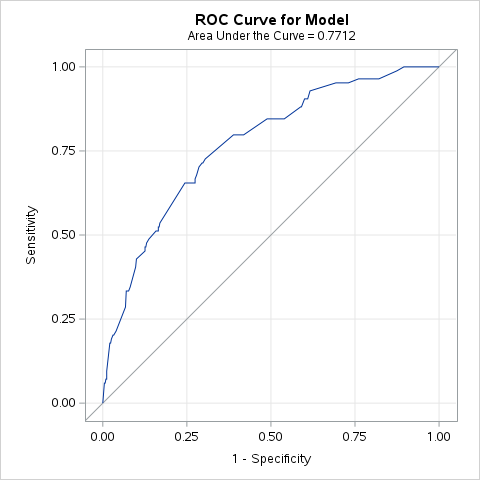
\includegraphics[width=0.45\textwidth,height=\textheight]{roc_model_a.png}
&
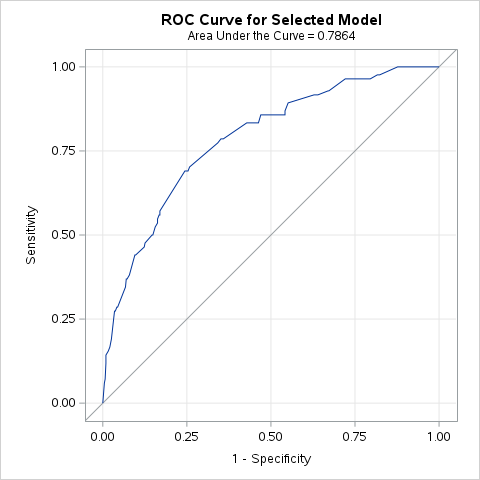
\includegraphics[width=0.45\textwidth,height=\textheight]{roc_model_b.png} \\
C-statistic = 0.771 & C-statistic = 0.786 \\
H-L Goodness-of-Fit p = 0.8742 & H-L Goodness-of-Fit p = 0.8311 \\
N of IPTW cohort = 514 & N of IPTW cohort = 514 \\
\bottomrule
\end{longtable}

\hypertarget{model-fit-statistics}{%
\subsection{Model Fit Statistics}\label{model-fit-statistics}}

\begin{longtable}[]{@{}lcc@{}}
\toprule
Criterion & Model A (No Interactions) & Model B (Interactions,
Backward) \\
\midrule
\endhead
C-statistic (AUC) & 0.771 & 0.786 \\
Hosmer-Lemeshow p-value & 0.8742 & 0.8311 \\
Full cohort size (IPTW) & 514 & 514 \\
\bottomrule
\end{longtable}

\hypertarget{balance-diagnostics-smd-after-iptw-weighting}{%
\subsection{Balance Diagnostics --- SMD After IPTW
Weighting}\label{balance-diagnostics-smd-after-iptw-weighting}}

The key criterion for selecting the final PS step 1 model is
\textbf{covariate balance after IPTW weighting}, measured by
standardized mean differences (SMD). An SMD \textless{} 0.10 indicates
good balance; SMD \textless{} 0.20 is acceptable for smaller samples.

\textbf{Standardized mean differences before and after IPTW weighting
--- Model A (ATE):}

\begin{longtable}[]{@{}clcc@{}}
\toprule
Obs & VarName & Stddiff (Before) & Stddiff (After IPTW) \\
\midrule
\endhead
1 & pneumo\_yes & −0.538 & −0.016 \\
2 & twin\_yes & 0.418 & −0.008 \\
3 & delivery\_vag & −0.398 & 0.002 \\
4 & inout\_transport & −0.494 & 0.049 \\
5 & bwt\_lt1000 & −0.354 & 0.104 \\
6 & bwt\_1000\_1299 & 0.079 & −0.124 \\
7 & gest\_lt28 & −0.448 & 0.015 \\
8 & gest\_28\_31 & 0.188 & −0.074 \\
& \textbf{Max \textbar SMD\textbar{}} & \textbf{0.538} &
\textbf{0.124} \\
\bottomrule
\end{longtable}

\textbf{Standardized mean differences before and after IPTW weighting
--- Model B (interactions, backward SLS = 0.20):}

\begin{longtable}[]{@{}clcc@{}}
\toprule
Obs & VarName & Stddiff (Before) & Stddiff (After IPTW) \\
\midrule
\endhead
1 & pneumo\_yes & −0.538 & −0.033 \\
2 & twin\_yes & 0.418 & −0.098 \\
3 & delivery\_vag & −0.398 & 0.040 \\
4 & inout\_transport & −0.494 & 0.043 \\
5 & bwt\_lt1000 & −0.354 & 0.070 \\
6 & bwt\_1000\_1299 & 0.079 & 0.162 \\
7 & gest\_lt28 & −0.448 & 0.042 \\
8 & gest\_28\_31 & 0.188 & 0.100 \\
& \textbf{Max \textbar SMD\textbar{}} & \textbf{0.538} &
\textbf{0.162} \\
\bottomrule
\end{longtable}

\hypertarget{final-model-selection-model-a}{%
\subsection{Final Model Selection: Model
A}\label{final-model-selection-model-a}}

I selected \textbf{Model A (no interactions)} as the final PS step 1
model. Model B had a slightly higher AUC (0.786 vs.~0.771), but the
weighted balance was better for Model A: the largest absolute SMD was
\textbf{0.124} for Model A compared with \textbf{0.162} for Model B.
Since the goal of the PS model is balance rather than prediction alone,
Model A was the better choice for this homework.

\hypertarget{model-a-parameter-estimates}{%
\subsection{Model A: Parameter
Estimates}\label{model-a-parameter-estimates}}

\begin{longtable}[]{@{}llccc@{}}
\toprule
Covariate & Level & OR & 95\% CI & p-value \\
\midrule
\endhead
Pneumothorax & Yes vs.~No & 3.712 & (2.073, 6.648) & \textless{}
0.001 \\
Multiple Gestation & Yes vs.~No & 0.319 & (0.136, 0.751) & 0.009 \\
Mode of Delivery & Vaginal vs.~C-Section & 2.178 & (1.234, 3.844) &
0.007 \\
Birth Location & Transport vs.~Duke & 2.571 & (1.458, 4.535) & 0.001 \\
Birth Weight & \textless{} 1000g vs.~\(\geq\) 1300g & 1.954 & (0.785,
4.861) & 0.150 \\
Birth Weight & 1000--1299g vs.~\(\geq\) 1300g & 1.564 & (0.711, 3.440) &
0.266 \\
Gestational Age & \textless{} 28 wks vs.~\(\geq\) 32 wks & 5.093 &
(1.028, 25.221) & 0.046 \\
Gestational Age & 28--31 wks vs.~\(\geq\) 32 wks & 5.063 & (1.145,
22.400) & 0.033 \\
\bottomrule
\end{longtable}

\emph{C-statistic = 0.771. Significant predictors of IVH: pneumothorax,
mode of delivery, birth location, and gestational age.}

\begin{center}\rule{0.5\linewidth}{0.5pt}\end{center}

\hypertarget{requirement-2-table-1-baseline-characteristics-before-and-after-iptw}{%
\section{Requirement 2: Table 1 --- Baseline Characteristics Before and
After
IPTW}\label{requirement-2-table-1-baseline-characteristics-before-and-after-iptw}}

IPTW for ATE was computed as follows:

\begin{itemize}
\tightlist
\item
  Treated (IVH = 1): \(w = 1 / \hat{e}\), where \(\hat{e}\) = propensity
  score
\item
  Control (IVH = 0): \(w = 1 / (1 - \hat{e})\)
\end{itemize}

These weights up-weight subjects whose covariate profile is ``unusual''
for their treatment group, creating a pseudo-population that mirrors the
overall covariate distribution in both exposure arms.

\hypertarget{table-1-baseline-characteristics-by-ivh-status-original-cohort-n-514}{%
\subsection{Table 1: Baseline Characteristics by IVH Status --- Original
Cohort (N =
514)}\label{table-1-baseline-characteristics-by-ivh-status-original-cohort-n-514}}

\begin{longtable}[]{@{}lcccc@{}}
\toprule
Covariate & No IVH (N = 430) & IVH (N = 84) & p-value & SMD
(Unweighted) \\
\midrule
\endhead
\textbf{Pneumothorax} & & & \textbf{\textless{} 0.001} & 0.538 \\
 No & 357 (83.0\%) & 50 (59.5\%) & & \\
 Yes & 73 (17.0\%) & 34 (40.5\%) & & \\
\textbf{Multiple Gestation} & & & 0.002 & 0.418 \\
 Singleton & 330 (76.7\%) & 77 (91.7\%) & & \\
 Multiple & 100 (23.3\%) & 7 (8.3\%) & & \\
\textbf{Mode of Delivery} & & & 0.001 & 0.398 \\
 C-Section & 221 (51.4\%) & 27 (32.1\%) & & \\
 Vaginal & 209 (48.6\%) & 57 (67.9\%) & & \\
\textbf{Birth Location} & & & \textbf{\textless{} 0.001} & 0.494 \\
 Born at Duke & 366 (85.1\%) & 54 (64.3\%) & & \\
 Transport & 64 (14.9\%) & 30 (35.7\%) & & \\
\textbf{Birth Weight Category} & & & 0.004 & 0.354 \\
 \textless{} 1000 g & 146 (34.0\%) & 43 (51.2\%) & & \\
 1000--1299 g & 170 (39.5\%) & 30 (35.7\%) & & \\
 1300--1599 g & 114 (26.5\%) & 11 (13.1\%) & & \\
\textbf{Gestational Age Category} & & & \textbf{\textless{} 0.001} &
0.448 \\
 \textless{} 28 weeks & 114 (26.5\%) & 40 (47.6\%) & & \\
 28--31 weeks & 255 (59.3\%) & 42 (50.0\%) & & \\
 \(\geq\) 32 weeks & 61 (14.2\%) & 2 (2.4\%) & & \\
\bottomrule
\end{longtable}

\emph{Column percentages and chi-square p-values are shown. In the
original cohort, the IVH and No-IVH groups were clearly different on all
six baseline covariates.}

\begin{center}\rule{0.5\linewidth}{0.5pt}\end{center}

\hypertarget{table-1-baseline-characteristics-by-ivh-status-ps-iptw-weighted-cohort-ate-n-514}{%
\subsection{Table 1: Baseline Characteristics by IVH Status --- PS-IPTW
Weighted Cohort (ATE, N =
514)}\label{table-1-baseline-characteristics-by-ivh-status-ps-iptw-weighted-cohort-ate-n-514}}

All 514 infants were retained in the IPTW analysis. ATE weights
(\(w = 1/\hat{e}\) for IVH = 1; \(w = 1/(1-\hat{e})\) for IVH = 0) were
applied. The weighted pseudo-population totals were 514.5 (No IVH) and
511.4 (IVH).

\begin{longtable}[]{@{}lcccccc@{}}
\toprule
Covariate & No IVH (Weighted N) & No IVH \% & IVH (Weighted N) & IVH \%
& p-value & Std Diff \\
\midrule
\endhead
\textbf{Total} & \textbf{514.5} & & \textbf{511.4} & & & \\
\textbf{Pneumothorax} & & & & & 0.779 & 0.016 \\
 No & 406.1 & 79.0\% & 400.0 & 78.2\% & & \\
 Yes & 108.3 & 21.1\% & 111.3 & 21.8\% & & \\
\textbf{Multiple Gestation} & & & & & 0.915 & 0.008 \\
 Singleton & 407.3 & 79.2\% & 403.5 & 78.9\% & & \\
 Multiple & 107.2 & 20.8\% & 107.9 & 21.1\% & & \\
\textbf{Mode of Delivery} & & & & & 0.979 & 0.002 \\
 C-Section & 248.0 & 48.2\% & 246.9 & 48.3\% & & \\
 Vaginal & 266.5 & 51.8\% & 264.4 & 51.7\% & & \\
\textbf{Birth Location} & & & & & 0.378 & 0.049 \\
 Born at Duke & 419.7 & 81.6\% & 427.8 & 83.7\% & & \\
 Transport & 94.8 & 18.4\% & 83.6 & 16.3\% & & \\
\textbf{Birth Weight Category} & & & & & 0.122 & 0.124 \\
 \textless{} 1000 g & 186.6 & 36.3\% & 159.6 & 31.2\% & & \\
 1000--1299 g & 202.3 & 39.3\% & 231.7 & 45.3\% & & \\
 1300--1599 g & 125.6 & 24.4\% & 120.0 & 23.5\% & & \\
\textbf{Gestational Age Category} & & & & & 0.252 & 0.074 \\
 \textless{} 28 weeks & 153.8 & 29.9\% & 149.3 & 29.2\% & & \\
 28--31 weeks & 297.8 & 57.9\% & 314.8 & 61.6\% & & \\
 \(\geq\) 32 weeks & 62.9 & 12.2\% & 47.2 & 9.2\% & & \\
\bottomrule
\end{longtable}

\emph{Weighted N and column percentages are shown. All p-values
\textgreater{} 0.05 indicate no statistically significant imbalance
after weighting. IPTW substantially reduced baseline imbalance; maximum
\textbar SMD\textbar{} = 0.124 (birth weight category).}

\textbf{Plain-language interpretation of Table 1:}

Before weighting, the IVH group and the No-IVH group were quite
different. Infants with IVH were generally more premature, had lower
birth weight, and were more likely to have pneumothorax. Because of
that, a crude comparison of mortality would mix the effect of IVH with
the effect of baseline illness severity.

After IPTW, the two groups looked much more similar. This means the
weighted comparison is fairer than the unadjusted comparison. Still, the
balance was not perfect, especially for birth-weight category, so the
IPTW estimate should be interpreted carefully.

\begin{center}\rule{0.5\linewidth}{0.5pt}\end{center}

\hypertarget{requirement-3-ps-and-iptw-weight-distribution}{%
\section{Requirement 3: PS and IPTW Weight
Distribution}\label{requirement-3-ps-and-iptw-weight-distribution}}

\hypertarget{propensity-score-distribution}{%
\subsection{Propensity Score
Distribution}\label{propensity-score-distribution}}

Under the final Model A, the propensity score ranged from \textbf{0.004
to 0.699}. As expected, infants with IVH had higher propensity scores
than infants without IVH (mean 0.286 vs.~0.139).

\begin{longtable}[]{@{}lcccccc@{}}
\toprule
Group & N & Mean PS & Median PS & SD & Min & Max \\
\midrule
\endhead
No IVH (IVH = 0) & 430 & 0.139 & 0.100 & 0.121 & 0.004 & 0.699 \\
IVH (IVH = 1) & 84 & 0.286 & 0.248 & 0.174 & 0.024 & 0.699 \\
\bottomrule
\end{longtable}

\hypertarget{iptw-weight-distribution}{%
\subsection{IPTW Weight Distribution}\label{iptw-weight-distribution}}

ATE weights are computed as \(w = 1/\hat{e}\) for IVH = 1 and
\(w = 1/(1-\hat{e})\) for IVH = 0. Subjects with extreme propensity
scores receive very large weights, potentially causing instability. All
weights were reviewed for extreme values.

\begin{longtable}[]{@{}lcccccc@{}}
\toprule
Group & N & Mean Weight & Median Weight & SD & Min & Max \\
\midrule
\endhead
No IVH (IVH = 0) & 430 & 1.196 & 1.112 & 0.263 & 1.004 & 3.320 \\
IVH (IVH = 1) & 84 & 6.088 & 4.033 & 7.031 & 1.431 & 41.940 \\
\bottomrule
\end{longtable}

\emph{The maximum weight for IVH-exposed infants was \textbf{41.94}.
This means a small number of observations had a large influence on the
weighted analysis. I did not truncate the weights in the main analysis,
but this is an important limitation.}

\hypertarget{scatter-plot-iptw-weight-vs.-estimated-propensity-score-ate}{%
\subsection{Scatter Plot: IPTW Weight vs.~Estimated Propensity Score
(ATE)}\label{scatter-plot-iptw-weight-vs.-estimated-propensity-score-ate}}

\begin{figure}
\centering
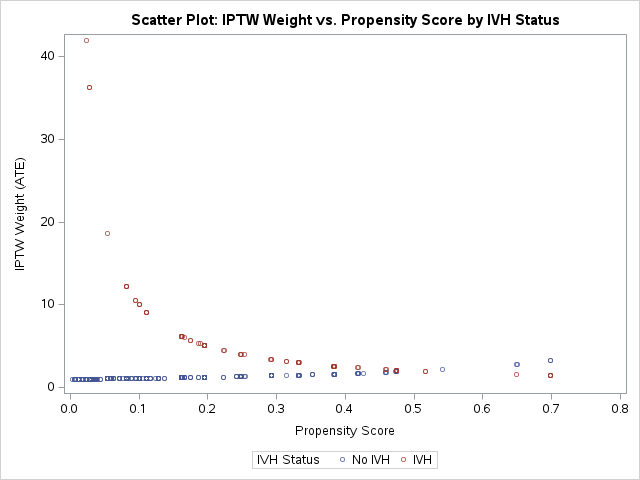
\includegraphics[width=0.8\textwidth,height=\textheight]{sgplot_1.png}
\caption{IPTW Weight vs Propensity Score}
\end{figure}

The scatter plot of IPTW weight versus propensity score illustrates the
inverse relationship between PS and weight within each exposure group:

\begin{itemize}
\tightlist
\item
  \textbf{IVH-exposed infants (IVH = 1):} Higher weights at lower
  propensity scores (infants unlikely to have IVH but who did). These
  cases are up-weighted because they provide information about the
  counterfactual outcome for ``low-risk'' infants.
\item
  \textbf{Unexposed infants (IVH = 0):} Higher weights at higher
  propensity scores (infants likely to have IVH who did not). These are
  up-weighted as they approximate the counterfactual for ``high-risk''
  infants.
\end{itemize}

\textbf{Plain-language interpretation:} The scatter plot shows that
infants with an exposure status that was less expected from their
baseline characteristics got larger weights. In this dataset, a few IVH
infants had especially large weights, so those cases had a strong effect
on the final IPTW estimate.

\begin{center}\rule{0.5\linewidth}{0.5pt}\end{center}

\hypertarget{requirement-4-table-2-comprehensive-comparison-of-effect-estimates}{%
\section{Requirement 4: Table 2 --- Comprehensive Comparison of Effect
Estimates}\label{requirement-4-table-2-comprehensive-comparison-of-effect-estimates}}

I compared four approaches for the IVH-mortality association:

\begin{enumerate}
\def\labelenumi{\arabic{enumi}.}
\tightlist
\item
  \textbf{Unadjusted:} Simple regression (no covariate adjustment).
\item
  \textbf{Adjusted (HW1):} Multivariable regression with purposeful
  variable selection (IVH + pneumothorax + bwt\_cat + gest\_cat).
\item
  \textbf{PS-Matched (HW3):} Conditional logistic regression / GEE
  Poisson, stratified on matched pair ID (164 infants, 82 pairs).
\item
  \textbf{PS-IPTW (HW4):} Weighted GEE with IPTW (ATE), full cohort N =
  514.
\end{enumerate}

\hypertarget{table-2-effect-estimates-ivh-vs.-no-ivh-on-mortality}{%
\subsection{Table 2: Effect Estimates --- IVH vs.~No IVH on
Mortality}\label{table-2-effect-estimates-ivh-vs.-no-ivh-on-mortality}}

\begin{longtable}[]{@{}
  >{\raggedright\arraybackslash}p{(\columnwidth - 8\tabcolsep) * \real{0.17}}
  >{\centering\arraybackslash}p{(\columnwidth - 8\tabcolsep) * \real{0.21}}
  >{\centering\arraybackslash}p{(\columnwidth - 8\tabcolsep) * \real{0.21}}
  >{\centering\arraybackslash}p{(\columnwidth - 8\tabcolsep) * \real{0.21}}
  >{\centering\arraybackslash}p{(\columnwidth - 8\tabcolsep) * \real{0.21}}@{}}
\toprule
& Dead = 0 & Dead = 1 & ORs (95\% CI) & RRs (95\% CI) \\
\midrule
\endhead
\textbf{IVH} & & & & \\
 No & 372 (86.5\%) & 58 (13.5\%) & Referent & Referent \\
 Yes & 43 (51.2\%) & 41 (48.8\%) & & \\
\textbf{Unadjusted} & & & 6.12 (3.67, 10.18) & 3.62 (2.43, 5.40) \\
\textbf{Adjusted ORs/RRs} & & & & \\
 Multivariable model (HW1 purposeful selection) & & & 4.15 (2.29, 7.52)
& 2.06 (1.35, 3.14) \\
 PS Matched (HW3, 82 pairs) & & & 3.86 (1.68, 8.86) & 2.05 (1.35,
3.12) \\
 \textbf{PS IPTW ATE (HW4)} & & & \textbf{3.34 (1.65, 6.76)} &
\textbf{2.45 (1.53, 3.90)} \\
\bottomrule
\end{longtable}

\emph{Dead = 0/1 counts show row percentages from the original
unweighted cohort (N = 514). Multivariable model (HW1): purposeful
selection includes IVH + pneumothorax + bwt\_cat + gest\_cat. PS
Matched: conditional logistic (OR) / GEE Poisson (RR), stratified on
MatchID. PS IPTW: GEE binomial logit (OR) / GEE Poisson log-link (RR)
with ATE weights and robust variance estimator. All estimates: p
\textless{} 0.001.}

\textbf{Plain-language interpretation of Table 2:}

\begin{itemize}
\item
  \textbf{Unadjusted (OR = 6.12; RR = 3.62):} In the crude analysis,
  infants with IVH had a much higher risk of death than infants without
  IVH. This estimate is probably too large because the IVH group was
  also sicker at baseline.
\item
  \textbf{Multivariable-adjusted, HW1 (OR = 4.15; RR = 2.06):} After
  adjusting for pneumothorax, birth weight, and gestational age, the
  estimate became smaller. This shows that confounding was important,
  but IVH still remained associated with about a two-fold higher risk of
  death.
\item
  \textbf{PS-Matched, HW3 (OR = 3.86; RR = 2.05):} The matched analysis
  gave almost the same RR as the HW1 adjusted model. That is helpful
  because two different adjustment methods gave very similar results.
\item
  \textbf{PS-IPTW ATE, HW4 (OR = 3.34; RR = 2.45):} The IPTW analysis
  also showed higher mortality in the IVH group. The weighted RR was a
  little larger than the HW1 and HW3 estimates, which may be related to
  the large IPTW weights and the remaining imbalance after weighting.
\item
  \textbf{Preferred measure and conclusion:} I prefer the \textbf{risk
  ratio} here because death is not a rare outcome in this dataset,
  especially among infants with IVH. The main IPTW estimate for this
  homework is \textbf{RR = 2.45 (95\% CI: 1.53, 3.90)}, but it should be
  read together with the evidence of extreme weights and some residual
  imbalance.
\end{itemize}

Overall, all four approaches point in the same direction: IVH is
associated with higher neonatal mortality in VLBW infants. The HW1
adjusted model and the HW3 matched model were very close to each other,
while the HW4 IPTW estimate was somewhat larger. For that reason, I
think the overall conclusion is stable, but the exact IPTW effect size
is less certain because of the large weights.

\begin{center}\rule{0.5\linewidth}{0.5pt}\end{center}

\hypertarget{summary}{%
\section{Summary}\label{summary}}

Using the main-effects PS model (Model A, C-statistic = 0.771), IPTW
improved covariate balance in the full cohort of 514 infants. After
weighting, all absolute SMDs were below 0.20, although birth-weight
category still showed the most residual imbalance (max
\textbar SMD\textbar{} = 0.124). The final IPTW estimate was RR = 2.45
(95\% CI: 1.53--3.90), which was in the same direction as the HW1 and
HW3 results but somewhat larger. My overall conclusion is that IVH is
associated with higher mortality, but the IPTW estimate should be
interpreted with caution because some weights were very large.

\end{document}
